\clearpage
\appendix
\renewcommand{\thefigure}{S.\arabic{figure}}
\renewcommand{\thetable}{S.\arabic{table}}
\renewcommand{\theequation}{S.\arabic{equation}}
\setcounter{figure}{0}
\setcounter{table}{0}
\setcounter{equation}{0}

\section{Further Training Details}\label{sec:further_training_details}
We finetune the LLaMA 1-based Vicuna 1.3 model\footnote{\url{https://huggingface.co/lmsys/vicuna-7b-v1.3}} with LoRA~\citep{hu2022lora}.
We use the HuggingFace Transformers and PEFT libraries, along with DeepSpeed \mbox{\texttt{ZeRO-2}}~\citep{zero}.
In all experiments, we use a \mbox{\texttt{lora\_r}} of \mbox{\texttt{128}}, a \mbox{\texttt{lora\_alpha}} of \mbox{\texttt{256}}, a LoRA learning rate of \mbox{\texttt{2e-05}}, a linear projector learning rate of \mbox{\texttt{2e-05}}, a numeric head learning rate of \mbox{\texttt{2e-04}}, and a cosine learning-rate schedule.
All models are trained with an effective batch size of \mbox{\texttt{32}} with \mbox{\texttt{bfloat16}} mixed-precision training.
Both the cross-entropy next-token-prediction and mean-square-error losses are given a weight of 1.

The models for the CLEVR and parameter-space generalization experiments are trained for \mbox{\texttt{40k}} steps.
The 6-DoF pose-estimation models are trained for \mbox{\texttt{200k}} steps.

We use the frozen CLIP visual tokenizer from \footnote{\url{https://huggingface.co/openai/clip-vit-large-patch14-336}}.
This CLIP variant has an input size of 336x336 pixels.
For the CLEVR evaluation, we render images at the original size of 480x320 to ensure compatibility with NS-VQA, but pad and resize them for use with our model.
For the remaining evaluations we directly render images at a resolution of 336x336.

We employ greedy token sampling across evaluations.

\section{Further CLEVR Data-Generation Details}
The original CLEVR dataset is rendered with random positional jitter in both the lights and camera.
This information is not recorded in the public dataset, so we re-render CLEVR-CoGenT with a fixed camera position, but maintain the randomness in the lighting.

\section{Further Numeric-Head Details}
Our numeric head is composed of a tanh layer, followed by a linear layer, a GELU activation, and a final linear projection.
The final LLaMA hidden state is passed through an RMS norm~\citep{rms_norm} before it is shared between the token head and numeric head, which re-scales but does not re-center the embedding.

During training, the locations of these tokens in the ground-truth sequence are known so they can be masked to apply the MSE loss.
During sampling, the position of these tokens is not pre-known and dependent on the generated sequence.
We first generate the token-only sequence and then substitute the estimated numbers back in with a second pass.

\begin{figure}[t!]
\centering
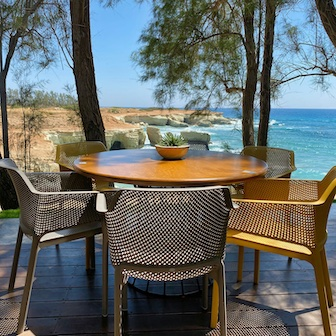
\includegraphics[width=0.2475\linewidth]{figures/shapenet/rw/0_in.jpg}\hfill
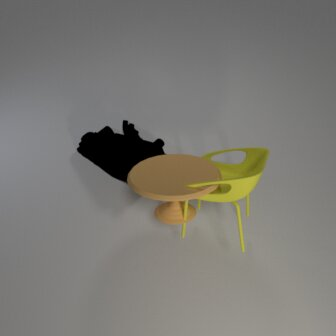
\includegraphics[width=0.2475\linewidth]{figures/shapenet/rw/0_out.jpg}\hfill
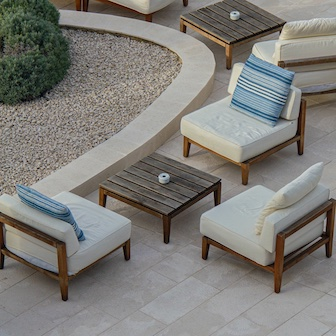
\includegraphics[width=0.2475\linewidth]{figures/shapenet/rw/1_in.jpg}\hfill
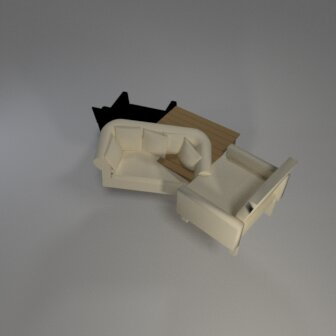
\includegraphics[width=0.2475\linewidth]{figures/shapenet/rw/1_out.jpg}
\caption{\textbf{Real-World ShapeNet 6-DoF Samples.} (\cref{sssec:scene_6dof}) 
Real-world sample reconstructions from the ShapeNet 6-Dof pose-estimation experiment.
We observe that the model is sensitive to OOD camera configurations.
During data generation, the camera is assigned a random pitch and radius, with its optical axis fixed passing through the global origin.
As such, we find that the model learns the bias and is limited by the expressivity of the training-data-generation framework, and, while it effectively interpolates values, it struggles to extrapolate outside of the camera configurations on which it was trained on.
We observe that the model is still, however, often able to identify the first few most-salient objects in the scene and produce meaningful assets (the first two in each of these samples being the rightmost chair then the table) before attempting to explain background features.
}
\label{fig:scene_6dof_rw_samples}
\end{figure}

\begin{table}
\centering
\caption{\textbf{Full CLEVR Data-Efficiency Results.} (\cref{ssec:clevr})}
\begin{subtable}[h]{0.495\linewidth}
\centering
\caption{ID}
{
\setlength{\tabcolsep}{2pt}
\begin{tabular}{lrrrrrr}
\toprule
 & $\downarrow$L2 & $\downarrow$Count & $\uparrow$Size & $\uparrow$Color & $\uparrow$Mat. & $\uparrow$Shape \\
\midrule
500 \\
\cline{1-1}
Char & 1.15 & \textbf{0.30} & 87.58 & 78.23 & 87.09 & 83.25 \\
Float & \textbf{0.98} & 0.44 & \textbf{91.43} & \textbf{85.51} & \textbf{90.73} & \textbf{89.29} \\
\hline
1000 \\
\cline{1-1}
Char & 0.73 & \textbf{0.18} & 97.14 & 94.54 & 96.50 & 95.98 \\
Float & \textbf{0.39} & \textbf{0.18} & \textbf{98.96} & \textbf{98.69} & \textbf{98.53} & \textbf{98.40} \\
\hline
2000 \\
\cline{1-1}
Char & 0.35 & \textbf{0.08} & \textbf{99.57} & \textbf{99.35} & \textbf{99.09} & \textbf{99.30} \\
Float & \textbf{0.26} & 0.09 & 99.55 & 99.28 & 99.04 & 99.23 \\
\hline
4000 \\
\cline{1-1}
Char & 0.21 & \textbf{0.05} & 99.71 & 99.58 & 99.27 & 99.51 \\
Float & \textbf{0.16} & \textbf{0.05} & \textbf{99.77} & \textbf{99.71} & \textbf{99.53} & \textbf{99.59} \\
\bottomrule
\end{tabular}
}
\label{table:clevr_efficiency_id}
\end{subtable}
\begin{subtable}[h]{0.495\linewidth}
\centering
\caption{OOD}
{
\setlength{\tabcolsep}{2pt}
\begin{tabular}{lrrrrrr}
\toprule
& $\downarrow$L2 & $\downarrow$Count & $\uparrow$Size & $\uparrow$Color & $\uparrow$Mat. & $\uparrow$Shape \\
\midrule
500 \\
\cline{1-1}
Char & 1.13 & \textbf{0.36} & 87.21 & 75.51 & 85.57 & 79.50 \\
Float & \textbf{1.01} & 0.53 & \textbf{90.71} & \textbf{79.45} & \textbf{89.24} & \textbf{84.42} \\
\hline
1000 \\
\cline{1-1}
Char & 0.74 & \textbf{0.21} & 96.25 & 92.19 & 94.87 & 90.45 \\
Float & \textbf{0.41} & 0.23 & \textbf{98.92} & \textbf{96.49} & \textbf{97.75} & \textbf{94.75} \\
\hline
2000 \\
\cline{1-1}
Char & 0.36 & \textbf{0.11} & \textbf{99.52} & \textbf{97.56} & \textbf{98.66} & 92.26 \\
Float & \textbf{0.28} & 0.12 & 99.29 & 97.33 & \textbf{98.66} & \textbf{94.76} \\
\hline
4000 \\
\cline{1-1}
Char & 0.22 & 0.06 & 99.74 & \textbf{98.60} & \textbf{99.33} & \textbf{93.50} \\
Float & \textbf{0.17} & \textbf{0.05} & \textbf{99.80} & 98.14 & 99.21 & 93.14 \\
\bottomrule
\end{tabular}
}
\label{table:clevr_ood_efficiency}
\end{subtable}
\label{table:clevr_data_efficiency}
\end{table}

\begin{table}[t]
\centering
\caption{
\textbf{CLEVR-CoGenT Results.} (\cref{ssec:clevr})
While both our proposed framework and the baseline, NS-VQA, and are able to achieve \textgreater 99\% accuracy on the ID condition, the baseline fails to generalize, with its shape-recognition accuracy dropping by 66.12\%.
\textit{Color}, \textit{Mat.}, and \textit{Shape} represent respective accuracies and $\uparrow$ indicates greater is better.
}
\begin{tabular}{lrrr|rrr}
\toprule
& \multicolumn{3}{c}{ID} & \multicolumn{3}{c}{OOD} \\
& Char & Float & NS-VQA & Char & Float & NS-VQA \\
\midrule
$\downarrow$L2 & 0.21 & 0.16 & 0.18 & 0.22 & 0.17 & 0.18 \\
$\uparrow$Size & 99.71 & 99.77 & 100.00 & 99.74 & 99.80 & 100.00 \\
$\uparrow$Color & 99.58 & 99.71 & 100.00 & 98.60 & 98.14 & 99.95 \\
$\uparrow$Shape & 99.51 & 99.59 & 100.00 & 93.50 & 93.14 & \fbox{33.88} \\
\bottomrule
\end{tabular}
\label{table:clevr}
\end{table}

\begin{figure}
\centering
\fbox{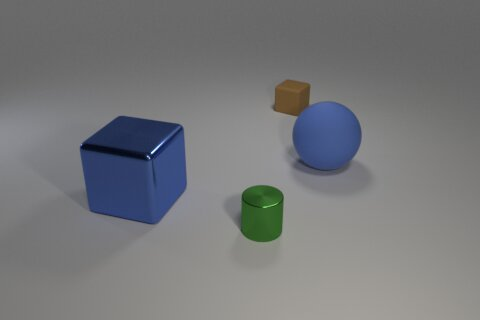
\includegraphics[width=0.533\linewidth]{figures/samples/clevr.jpg}}
\begin{minted}[breaklines]{python}
add(color='green', size='tiny', material='shiny', shape='cylinder', loc=(2.163, -1.384, 0.350))
add(material='metal', rotation=-0.126, shape='cube', loc=(-0.033, -2.456, 0.700), color='blue', size='large')
add(size='large', material='rubber', color='blue', loc=(1.352, 1.165, 0.700), shape='sphere')
add(color='brown', material='matte', shape='cube', size='tiny', loc=(-1.185, 2.816, 0.350), rotation=0.144)
\end{minted}
\caption{\textbf{CLEVR-CoGenT Train Sample.} (\cref{ssec:clevr})}
\label{fig:code_clevr}
\end{figure}
\begin{figure*}[t]
\centering
\begin{subfigure}{.196\linewidth}
\centering
\raisebox{0cm}{
\includegraphics[width=\linewidth]{figures/2d/sparse_checkerboard.pdf}}
\caption{Train Distribution}\label{fig:2d_sparse_checkerboard}
\end{subfigure}
\hspace{-0.15cm}
\begin{subfigure}{.196\linewidth}
\centering
\raisebox{0cm}{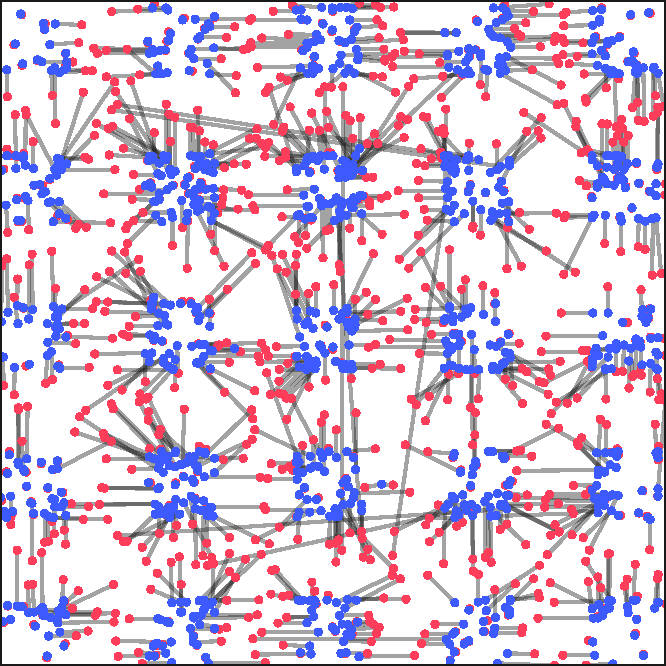
\includegraphics[width=\linewidth]{figures/2d/char_scatter.pdf}}
\caption{Char Model Pred.}\label{fig:2d_char_scatter}
\end{subfigure}
\hspace{-0.15cm}
\begin{subfigure}{.196\linewidth}
\centering
\raisebox{0cm}{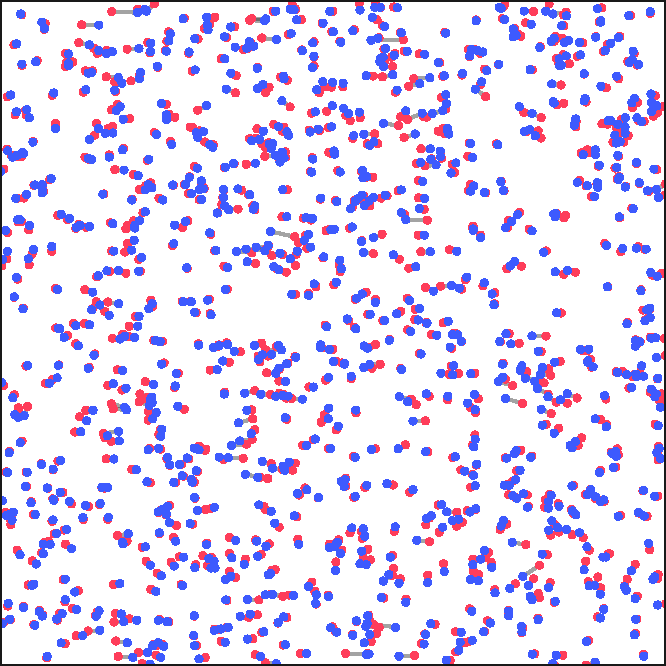
\includegraphics[width=\linewidth]{figures/2d/float_scatter.pdf}}
\caption{Float Model Pred.}\label{fig:2d_float_scatter}
\end{subfigure}
\begin{subfigure}{.196\linewidth}
\centering
\raisebox{0.0cm}{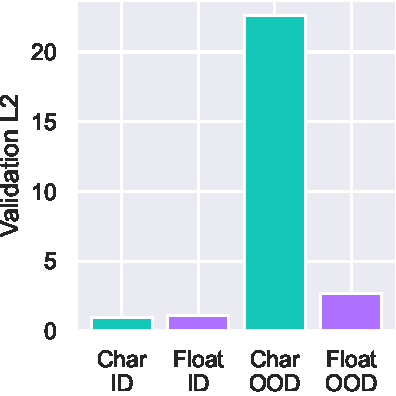
\includegraphics[width=\linewidth]{figures/2d/bar.pdf}}
\caption{ID--OOD}
\label{fig:2d_bar}
\end{subfigure}
\hfill
\begin{subfigure}{.196\linewidth}
\centering
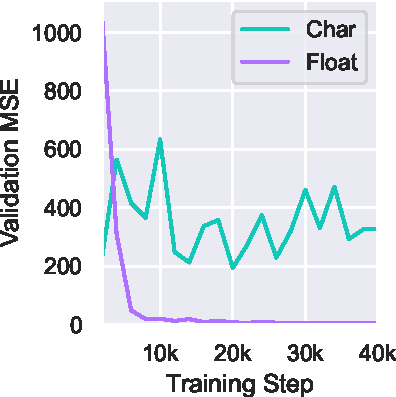
\includegraphics[width=\linewidth]{figures/2d/dynamics.pdf}
\caption{Dynamics}
\label{fig:2d_dynamics}
\end{subfigure}
\caption{\textbf{2D Parameter-Space Generalization.} (\cref{sssection:2d})
(a) Training positions are sampled from the checkerboard.
When evaluated on images with uniformly sampled positions, the char-based model fails to generalize outside the training distribution (b) while the float-based model effectively interpolates samples (c).
Randomly-sampled testing locations are shown in red and the corresponding predictions in blue.
(d) shows that while both methods well-estimate samples from the ID condition, the char-based model struggles to generalize.
(e) shows a plot of the model's validation MSE as a function of the number of training steps.
We observe that the training of the float-based model is much smoother and converges quickly.
}
\label{fig:2d}
\end{figure*}
\begin{figure}
\centering
\fbox{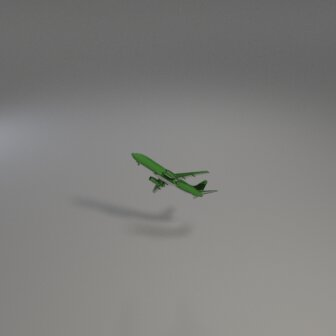
\includegraphics[width=0.4\linewidth]{figures/samples/so3.jpg}}
\begin{minted}[breaklines]{python}
add(shape='airliner', size='tiny', color='green', material='matte', rotation=(-0.798, 0.124, 0.590, -0.562, -0.507, -0.654))
\end{minted}
\caption{\textbf{SO(3) Range-Gap Train Sample.} (\cref{sssec:so3})}
\label{fig:code_so3}
\end{figure}
\begin{figure}
\centering
\fbox{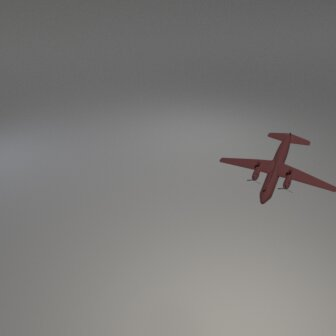
\includegraphics[width=0.4\linewidth]{figures/samples/single_object_6dof.jpg}}
\begin{minted}[breaklines]{python}
add(loc=(6.355, -4.600, 4.206), color='Mahogany', shape='jet', material='matte', rotation=(0.941, -0.337, 0.022, -0.303, -0.815, 0.493))
\end{minted}
\caption{\textbf{Single-Object 6-DoF Train Sample.} (\cref{sssec:single_6dof})}
\label{fig:code_single_6dof}
\end{figure}
\begin{figure}
\centering
\fbox{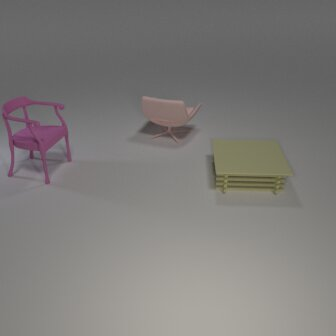
\includegraphics[width=0.4\linewidth]{figures/samples/scene_level_6dof.jpg}}
\begin{minted}[breaklines]{python}
add(rotation=(0.999, 0.024, -0.042, 0.024, 0.496, 0.868), color='Olive Green', loc=(2.228, 0.057, -10.362), shape='tables_0010')
add(rotation=(0.934, 0.177, -0.310, 0.163, 0.561, 0.812), loc=(0.032, 1.816, -12.639), color='Melon', shape='chairs_0055')
add(loc=(-3.707, 1.009, -10.332), rotation=(-0.235, 0.481, -0.845, -0.689, -0.696, -0.204), shape='chairs_0008', color='Red Violet')
\end{minted}
\caption{\textbf{ShapeNet 6-DoF Train Sample.} (\cref{sssec:scene_6dof})}
\label{fig:code_scene_6dof}
\end{figure}

\begin{figure}
\centering
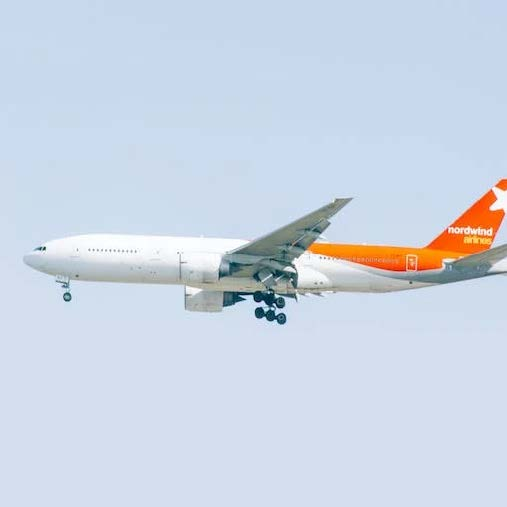
\includegraphics[width=0.2475\linewidth]{figures/airplane/6dof/input/2.jpg}\hfill
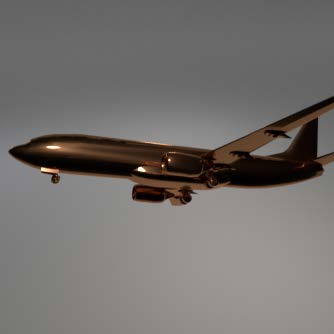
\includegraphics[width=0.2475\linewidth]{figures/airplane/6dof/output/2.jpg}\hfill

\includegraphics[width=0.2475\linewidth]{figures/airplane/6dof/input/3.jpg}\hfill

\includegraphics[width=0.2475\linewidth]{figures/airplane/6dof/output/3.jpg}
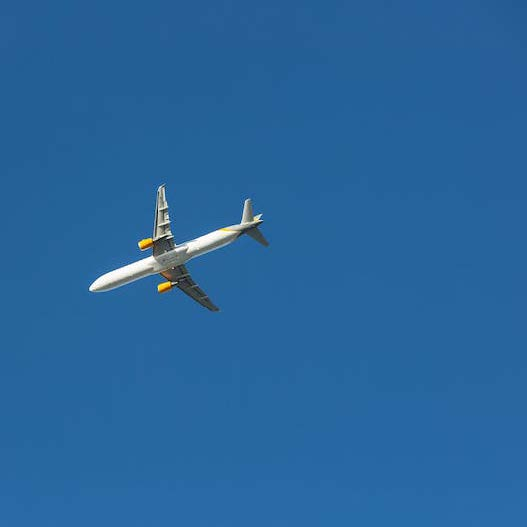
\includegraphics[width=0.2475\linewidth]{figures/airplane/6dof/input/4.jpg}\hfill
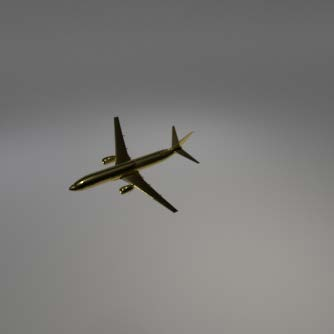
\includegraphics[width=0.2475\linewidth]{figures/airplane/6dof/output/4.jpg}\hfill

\includegraphics[width=0.2475\linewidth]{figures/airplane/6dof/input/5.jpg}\hfill
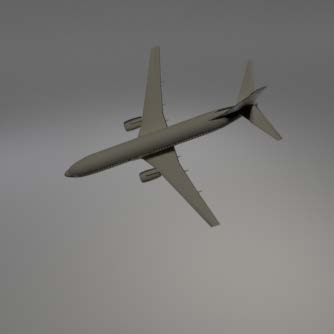
\includegraphics[width=0.2475\linewidth]{figures/airplane/6dof/output/5.jpg}
\caption{\textbf{Additional OOD Single-Object 6-DoF Samples.} (\cref{sssec:single_6dof})
Input--output pairs are shown left-to-right.
}
\label{fig:single_6dof_samples_additional}
\end{figure}
\begin{figure}
\centering
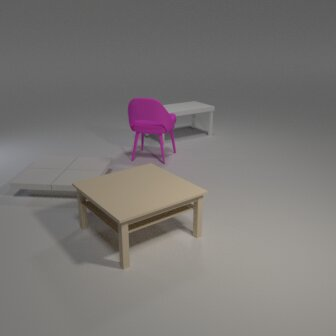
\includegraphics[width=0.2475\linewidth]{figures/shapenet/ID/0_in.jpg}\hfill
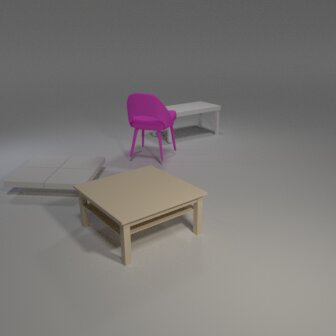
\includegraphics[width=0.2475\linewidth]{figures/shapenet/ID/0_out.jpg}\hfill
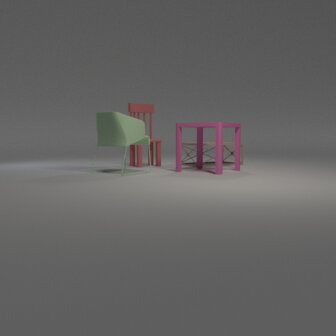
\includegraphics[width=0.2475\linewidth]{figures/shapenet/ID/1_in.jpg}\hfill
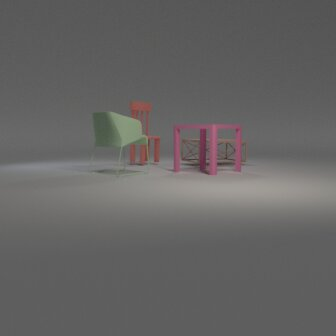
\includegraphics[width=0.2475\linewidth]{figures/shapenet/ID/1_out.jpg}
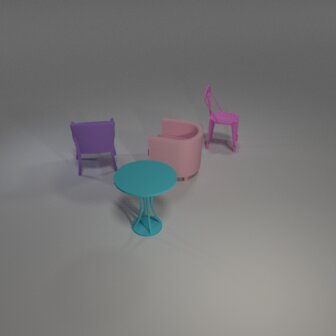
\includegraphics[width=0.2475\linewidth]{figures/shapenet/ID/2_in.jpg}\hfill
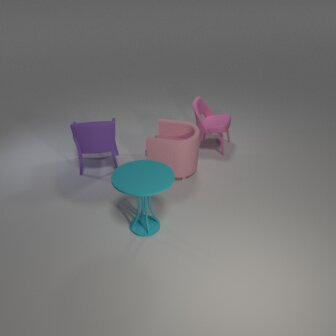
\includegraphics[width=0.2475\linewidth]{figures/shapenet/ID/2_out.jpg}\hfill
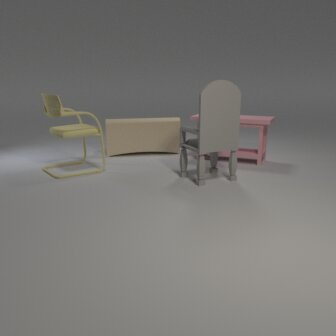
\includegraphics[width=0.2475\linewidth]{figures/shapenet/ID/3_in.jpg}\hfill
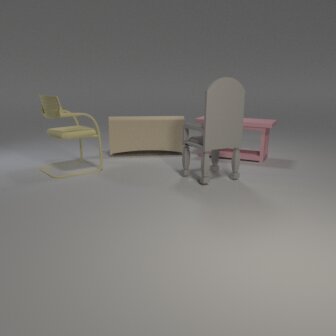
\includegraphics[width=0.2475\linewidth]{figures/shapenet/ID/3_out.jpg}
\caption{\textbf{ID ShapeNet 6-DoF Samples.} (\cref{sssec:scene_6dof}) Input--output pairs are shown left-to-right.}
\label{fig:scene_6dof_id_samples_additional}
\end{figure}

\begin{figure}
\centering
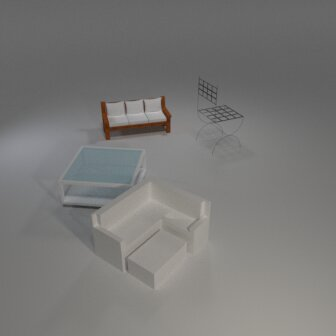
\includegraphics[width=0.2475\linewidth]{figures/shapenet/OOD/2_in.jpg}\hfill
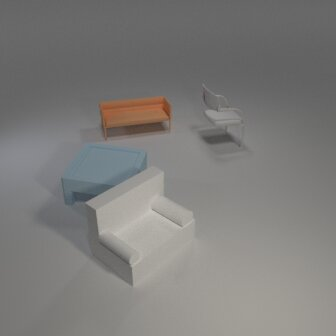
\includegraphics[width=0.2475\linewidth]{figures/shapenet/OOD/2_out.jpg}\hfill
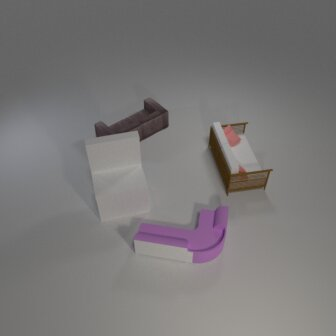
\includegraphics[width=0.2475\linewidth]{figures/shapenet/OOD/3_in.jpg}\hfill
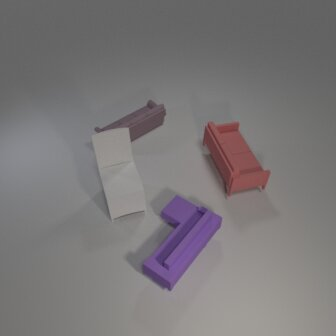
\includegraphics[width=0.2475\linewidth]{figures/shapenet/OOD/3_out.jpg}
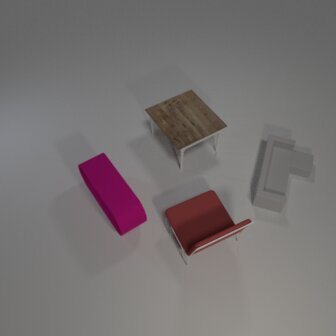
\includegraphics[width=0.2475\linewidth]{figures/shapenet/OOD/4_in.jpg}\hfill
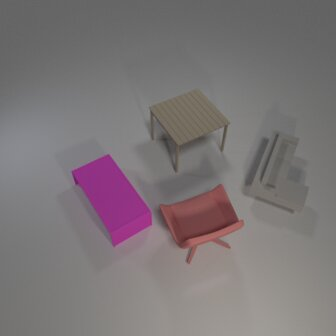
\includegraphics[width=0.2475\linewidth]{figures/shapenet/OOD/4_out.jpg}\hfill
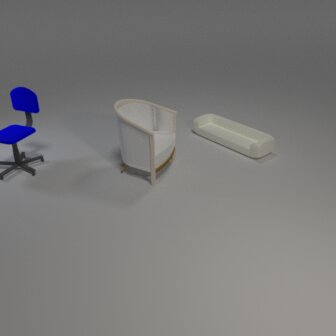
\includegraphics[width=0.2475\linewidth]{figures/shapenet/OOD/5_in.jpg}\hfill
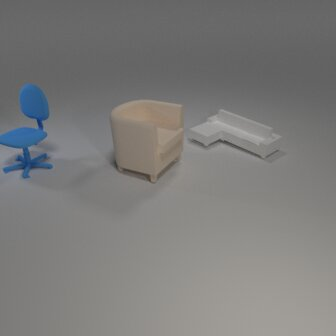
\includegraphics[width=0.2475\linewidth]{figures/shapenet/OOD/5_out.jpg}
\caption{\textbf{Additional OOD ShapeNet 6-DoF Samples.} (\cref{sssec:scene_6dof}) Input--output pairs are shown left-to-right.}
\label{fig:scene_6dof_ood_samples_additional}
\end{figure}

\begin{figure}
\centering
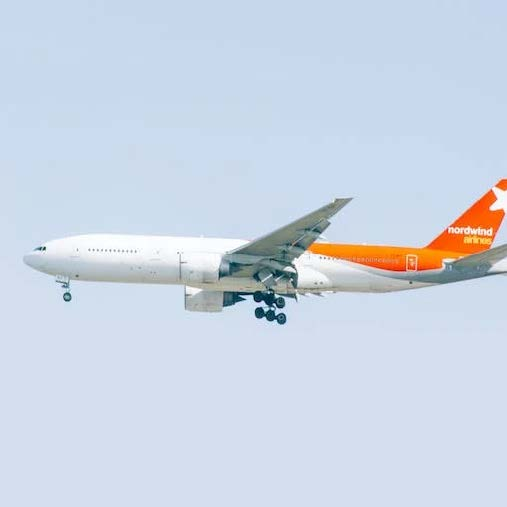
\includegraphics[width=0.2475\linewidth]{figures/airplane/6dof/input/2.jpg}\hfill
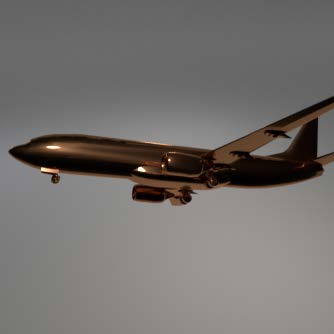
\includegraphics[width=0.2475\linewidth]{figures/airplane/6dof/output/2.jpg}\hfill

\includegraphics[width=0.2475\linewidth]{figures/airplane/6dof/input/3.jpg}\hfill

\includegraphics[width=0.2475\linewidth]{figures/airplane/6dof/output/3.jpg}
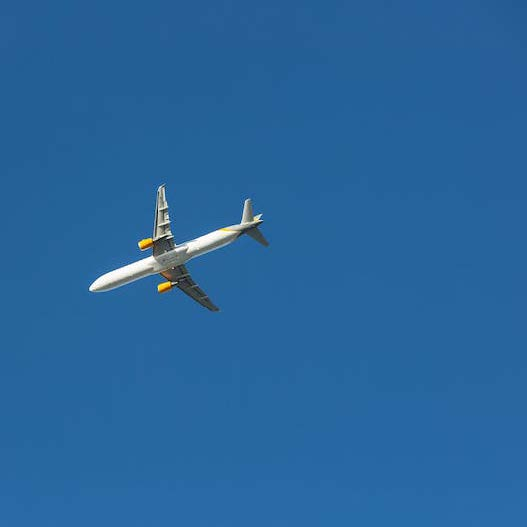
\includegraphics[width=0.2475\linewidth]{figures/airplane/6dof/input/4.jpg}\hfill
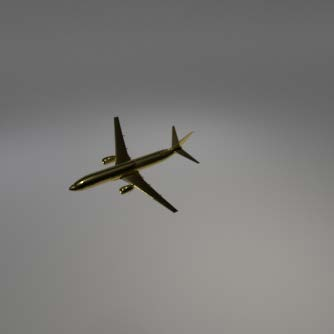
\includegraphics[width=0.2475\linewidth]{figures/airplane/6dof/output/4.jpg}\hfill

\includegraphics[width=0.2475\linewidth]{figures/airplane/6dof/input/5.jpg}\hfill
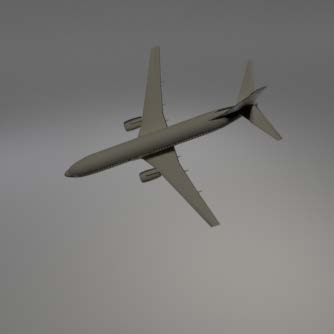
\includegraphics[width=0.2475\linewidth]{figures/airplane/6dof/output/5.jpg}
\caption{\textbf{Additional OOD Single-Object 6-DoF Samples.} (\cref{sssec:single_6dof})
Input--output pairs are shown left-to-right.
}
\label{fig:single_6dof_samples_additional}
\end{figure}